\chapter{Introduction}

Signal processing has long relied on well-defined, structured processes and protocols to function.  However, in order to move to more robust and adaptive systems, we will need to overhaul these tightly structured processes.  We must design new robust and adaptive communications systems.

From an academic perspective, the rise of machine learning tools and processing has allowed us to tackle problems we have not yet been able to, like in image processing.  However, we still do not fully understand the reach or the limitations of this technology.  In order to study the limitations of machine learning, we must apply them to spaces that we have studied extensively, like communications, and compare them to the well-known baselines.

Most communications systems have three main processes at the receiver; equalization, demodulation, and error-correction.  While we will need to design robust forms of all of these processes, we will focus on equalization for the remainder of this paper. 

\section{Motivation}

Meta-learning is the idea that algorithms need to be able to `learn to learn' in order to generalize to different applications.  For example, if a robot is trained to pick up coffee mugs, then we want that robot to be able to quickly learn how to pick up water bottles without having to re-train it.  
Meta-learning was inspired by humans ability to generalize how to learn \cite{lake}.  
Additionally, researchers in neurology have studied how the brain synapses change over time, suggesting that our algorithms will have to change over time to continue learning \cite{bengio}.
We refer the reader to \cite{lemke} for a survey of meta-learning technologies and to \cite{finn} for recent developments in meta-learning algorithms.

In this paper, we want to understand if our neural network based communication processes can learn to learn.  
As in, can they handle new environments with new data sequeneces without having to re-train for the new variables. 
The communications application is arguably an easier application of meta-learning than others have been exploring, like image classification \cite{khodadeh}.  
In order to better understand the reach and limitations of meta-learning, we need to apply it to something simpler, like communications.  In this paper, we will explore whether or not we can learn to learn to communicate. 

\section{Background}

\subsection{Inter-symbol Interference and Equalization}

Inter-symbol interference occurs when we are transmitting over a channel that has some echos.  These echos cause the receiver to hear a garbled signal instead of the original signal from the transmitter.  This is called inter-symbol interference because the receiver is hearing a combination of symbols across time. 

Let $\vec{x}=[x_0, x_1, \ldots x_n]$ be the set of $n$ complex symbols that the transmitter sends over the channel that connects the transmitter to the receiver.
Each channel will have different characteristics. Some channels may have echos, others may have delays, often channels will have both.  When a channel has echos, this is called a multipath channel because there are multiple paths to reach the receiver.  Each path is called a tap.  We can characterize a channel by characterizing the taps.

Let $\vec{a} = [a_0, a_1, \ldots a_{\ell}]$ be the set of characteristic for a multipath channel that has $l$ taps. When a sequence of symbols like $\vec{x}$ is transmitted over this channel, the channel taps are convolved over the sequence.  Additionally, there is noise in the system denoted by $v_i$. 

\begin{align}
\tilde{x}_m = \sum_{i=0}^{\ell} a_i x_{m-i} + v_i
\end{align}

The receiver will hear a signal that is corrupted by inter-symbol interfence and noise;
$\vec{\tilde{x}}=[\tilde{x}_0, \tilde{x_1}, \ldots \tilde{x}_{n+\ell}]$. 
Receivers must be able to handle garbled signals in order to transmit data in the real world.  The process of removing the inter-symbol interference is called equalization.  The goal of equalization is to take in a garbled signal and output a signal with minimal inter-symbol interference. 

\setlength{\tabcolsep}{0pt}
\begin{figure}
  \centering
  \caption{The effects of a two tap channel on the QPSK constellation.}
  \begin{tabular}{ccc}
    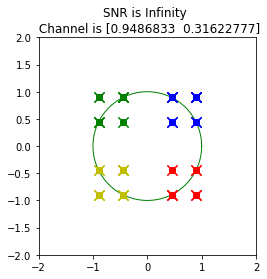
\includegraphics[width=45mm]{figures/equal_intro/snr_0_c3/cfo_0.png}&
    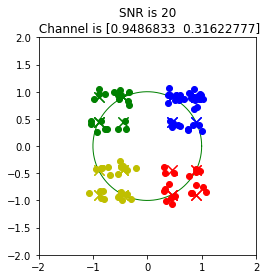
\includegraphics[width=45mm]{figures/equal_intro/snr_20_c3/cfo_0.png}&
    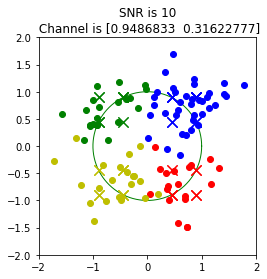
\includegraphics[width=45mm]{figures/equal_intro/snr_10_c3/cfo_0.png}\\
    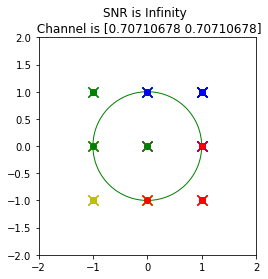
\includegraphics[width=45mm]{figures/equal_intro/snr_0_c2/cfo_0.png}&
    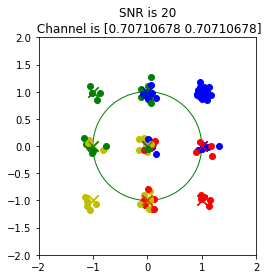
\includegraphics[width=45mm]{figures/equal_intro/snr_20_c2/cfo_0.png}&
    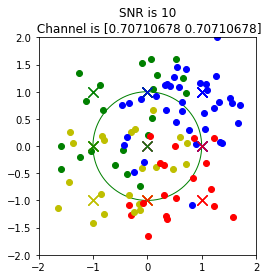
\includegraphics[width=45mm]{figures/equal_intro/snr_10_c2/cfo_0.png}\\
    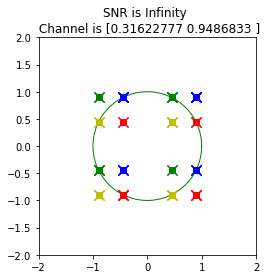
\includegraphics[width=45mm]{figures/equal_intro/snr_0_c4/cfo_0.png}&
    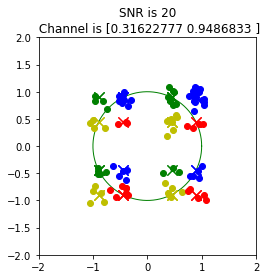
\includegraphics[width=45mm]{figures/equal_intro/snr_20_c4/cfo_0.png}&
    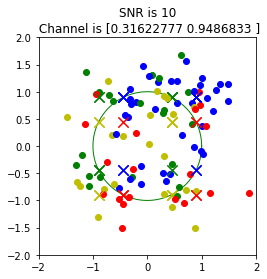
\includegraphics[width=45mm]{figures/equal_intro/snr_10_c4/cfo_0.png}\\
    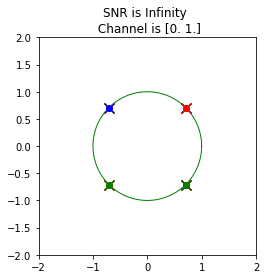
\includegraphics[width=45mm]{figures/equal_intro/snr_0_c5/cfo_0.png}&
    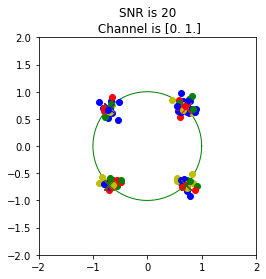
\includegraphics[width=45mm]{figures/equal_intro/snr_20_c5/cfo_0.png}&
    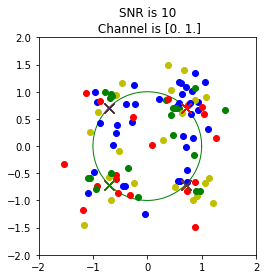
\includegraphics[width=45mm]{figures/equal_intro/snr_10_c5/cfo_0.png}\\
  \end{tabular}
  \label{fig:multi_tap}
\end{figure}

Figure ~\ref{fig:multi_tap} demonstrates the effects of multi-tap channels on a QPSK modulation constellation.  
We show what the received signal symbols constellations are from a sequence of $100$ symbols modulated in QPSK through different two tap channels.  We assume that the channel taps are constant during the transmission of the signal.
We see that under certain channel conditions, like when the two taps are equal, it is very difficult to distinguish between the four constellations.  
Engineers have built processes to remove inter-symbol interference.  First, let's go into the case when the channel characteristics are known.

\subsubsection{Equalization for a known channel}

If the receiver knows the channel characteristics, $\vec{a}$, perfectly, then there are a few different methods that can be used.  
The zero-forcing equalizer applies the inverse of the channel response to the received signal.  It is called zero-forcing because there will be zero inter-symbol interference if there is no noise.
There are some limitations of the zero-forcing equalizer. 
First, the impulse response of the equalizer needs to be infinitely long. 
Second, if there is a weak signal at a frequency, then the inverse gain is going to be very large.  This will amplify any noise in the system. 
Third, if there are any zeros in frequency response, these cannot be inverted.

Another equalizer, the minimum mean squared error (MMSE) equalizer, handles noise much better than the zero-forcing equalizer and is explained in the next section.
While it's important to consider how well a receiver can equalize with a known channel, this is rarely the case.  Usually, we do not know the channel characteristics.

\subsubsection{Equalization for an unknown channel}
When the receiver does not know the channel characteristics, the process of equalization essentially has two jobs; first, identify the channel, second, remove the inter-symbol interference. If the receiver did not identify the channel first, there would be no way to remove the affects of it on the received signal. 

In order to do channel estimation, most systems require that packets begin with a known sequence called a preamble. The signal sent will be broken into two parts; $\vec{x} = [\vec{x}_{pre}, \vec{x}_{data}]$.  The signal received on the transmitter is $\vec{\tilde{x}}=[\vec{\tilde{x}}_{pre},\vec{\tilde{x}}_{data}]$.  
The receiver knows what the orginal preamble sequence was, $\vec{x}_{pre}$, and can use the received preamble sequence, $\vec{\tilde{x}}_{pre}$, to estimate the behavior of the channel.
Once the channel is estimated, the receiver then equalizes the data, $\vec{\tilde{x}}_{data}$.

One common method to estimate the channel is to use the least squares optimization framework. Let $H$ be the estimate of the channel.  The least squares channel estimator wants to find $H$ that minimizes the squared error between the received signal, $\vec{\tilde{x}}_{pre}$, and what the predicted received signal would be if the the channel $H$ was applied to the original preamble, $\vec{x}_{pre}$.
\begin{align}
\min_H ||\vec{\tilde{x}}_{pre}-H\vec{x}_{pre}||^2
\end{align}

The receiver needs to choose the length of $H$, representing how many taps (or echos) there might be in the channel.  The length of $H$ will be set based on the environment that the transmitter and receiver are communicating in.

Once the channel response has been estimated, an equalizer has to use that information to remove the inter-symbol interference from the received signal.
The MMSE equalizer minimizes the error between the equalized preamble and the original known preamble by choosing the optimal inverse of the channel response, $W$.
\begin{align}
\min_W||\vec{x}_{pre}-\vec{\hat{x}}_{pre}||^2 \\
\vec{\hat{x}}_{pre} = W (H\vec{x}_{pre}+\vec{v}) \\
W^* = \vec{x}_{pre} \vec{x}_{pre}^T H^T (H \vec{x}_{pre} \vec{x}_{pre}^T H^T + \sigma_v^2 I)^{-1}
\end{align}

The MMSE equalizer works well for known and unknown channels and does not amplify noise like the zero-forcing equalizer.  This is why the MMSE equalizer paired with a least squares channel estimator are widely used.

 
\subsection{Carrier Frequency Offset and Correction}

\setlength{\tabcolsep}{0pt}
\begin{figure}
  \centering
  \caption{The effects of a carrier frequency offset on the QPSK constellation.}
  \begin{tabular}{ccc}
    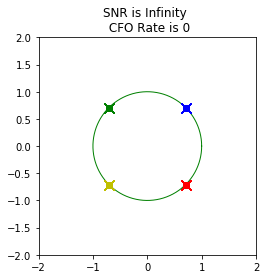
\includegraphics[width=50mm]{figures/cfo_intro/snr_0/cfo_0.png}&
    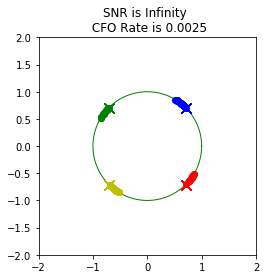
\includegraphics[width=50mm]{figures/cfo_intro/snr_0/cfo_1.png}&
    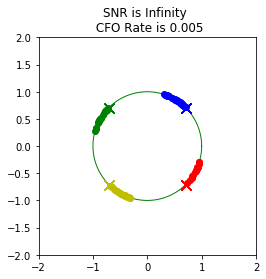
\includegraphics[width=50mm]{figures/cfo_intro/snr_0/cfo_2.png}\\
    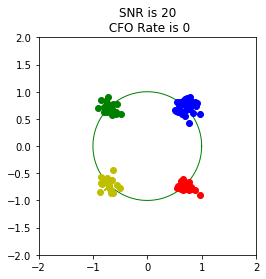
\includegraphics[width=50mm]{figures/cfo_intro/snr_20/cfo_0.png}&
    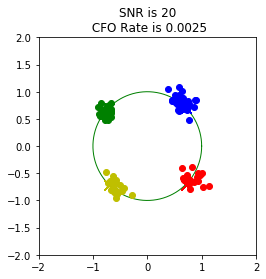
\includegraphics[width=50mm]{figures/cfo_intro/snr_20/cfo_1.png}&
    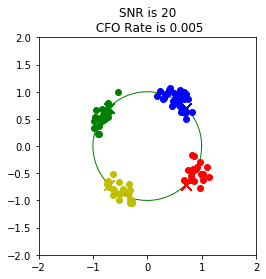
\includegraphics[width=50mm]{figures/cfo_intro/snr_20/cfo_2.png}\\
    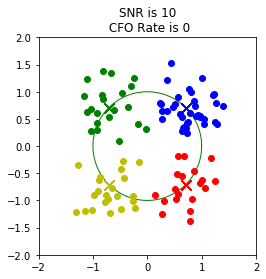
\includegraphics[width=50mm]{figures/cfo_intro/snr_10/cfo_0.png}&
    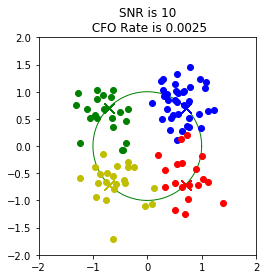
\includegraphics[width=50mm]{figures/cfo_intro/snr_10/cfo_1.png}&
    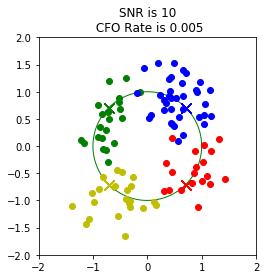
\includegraphics[width=50mm]{figures/cfo_intro/snr_10/cfo_2.png}
  \end{tabular}
  \label{fig:single_tap_cfo}
\end{figure}

Now, if we were to implement our minimum mean squared error equalizer on a physical receiver, we would find some problems with our equalization process.  
Our equalizer will equalize the first symbols very well.  However, as we equalize end parts of our sequence, we will encounter a physical phenomonen called carrier frequency offset, CFO.
Carrier frequency offset occurs when the transmitter and receiver are at slightly different frequencies.  It also occurs when the transmitter and receiver are moving, causing a sort of Doppler effect. 

When there is a significant CFO present, the symbols will gradually rotate. The received signals will be the original signals rotated at a rate $\omega$.
\begin{align}
\tilde{x}_i = x_i e^{ij\omega}+v_i
\end{align} 

Figure ~\ref{fig:single_tap_cfo} demonstrates the effects of CFO on a QPSK modulation constellation (no multipath channels). 
We show what the received signal symbols constellations are from a sequence of $100$ symbols modulated in QPSK with different CFO rates.  We assume that the CFO rate, $\omega$, is constant during the transmission of the signal.

There are a few ways to handle CFO, some are more elegant than others. 
The first solution is to try to side-step the problem entirely.  
Since the effects of CFO depend on the length of a packet, one solution is to make packets so short that the symbols only move a little bit.  In this case, the effects of CFO can be ignored.

Another solution is using a phase-locked loop, which is a control system that outputs a signal with a phase related to the input signal.  
A Costas loop is a circuit that implements a phase-locked loop for CFO correction for continuous time signals by adapting the sampling rate \cite{costas}.

\setlength{\tabcolsep}{0pt}
\begin{figure}
  \centering
  \caption{The effects of a two tap channel and a carrier frequency offset on the QPSK constellation.}
  \begin{tabular}{ccc}
    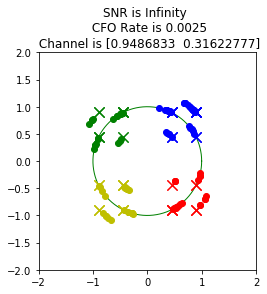
\includegraphics[width=45mm]{figures/cfo_equal_intro/snr_0_c3/cfo_0.png}&
    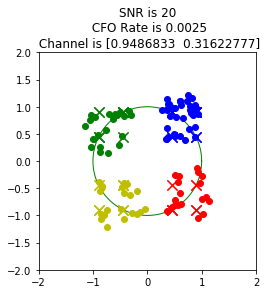
\includegraphics[width=45mm]{figures/cfo_equal_intro/snr_20_c3/cfo_0.png}&
    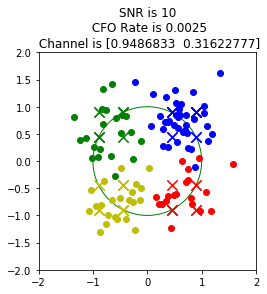
\includegraphics[width=45mm]{figures/cfo_equal_intro/snr_10_c3/cfo_0.png}\\
    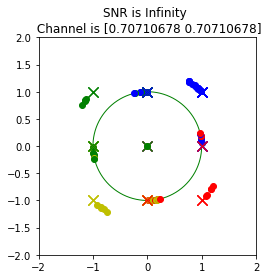
\includegraphics[width=45mm]{figures/cfo_equal_intro/snr_0_c2/cfo_0.png}&
    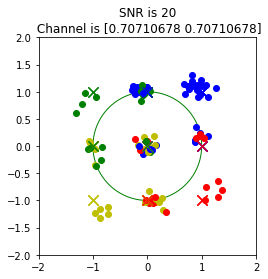
\includegraphics[width=45mm]{figures/cfo_equal_intro/snr_20_c2/cfo_0.png}&
    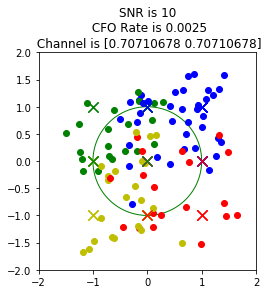
\includegraphics[width=45mm]{figures/cfo_equal_intro/snr_10_c2/cfo_0.png}\\
    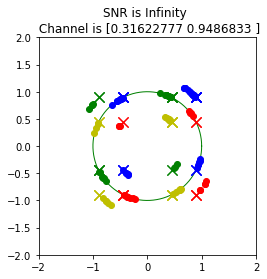
\includegraphics[width=45mm]{figures/cfo_equal_intro/snr_0_c4/cfo_0.png}&
    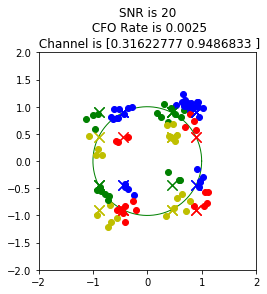
\includegraphics[width=45mm]{figures/cfo_equal_intro/snr_20_c4/cfo_0.png}&
    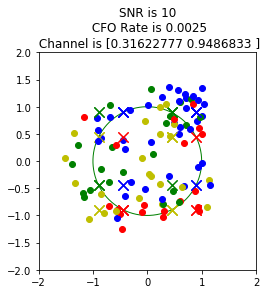
\includegraphics[width=45mm]{figures/cfo_equal_intro/snr_10_c4/cfo_0.png}\\
    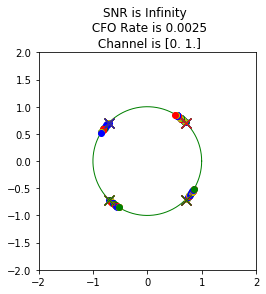
\includegraphics[width=45mm]{figures/cfo_equal_intro/snr_0_c5/cfo_0.png}&
    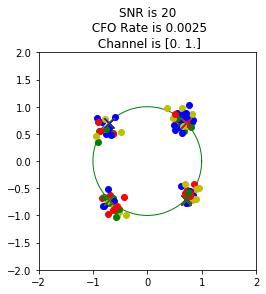
\includegraphics[width=45mm]{figures/cfo_equal_intro/snr_20_c5/cfo_0.png}&
    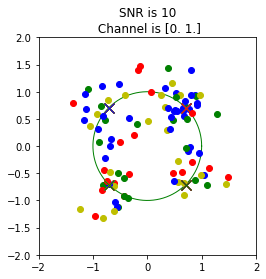
\includegraphics[width=45mm]{figures/cfo_equal_intro/snr_10_c5/cfo_0.png}\\
  \end{tabular}
  \label{fig:multi_tap_cfo}
\end{figure}

What happens when there is both CFO and inter-symbol interference?  The received signal will have the effects of the channel and CFO as well as the noise. 

\begin{align}
\tilde{x}_m = (\sum_{i=0}^l a_i x_{m-i})e^{mj\omega} + v_i
\end{align}

Figure ~\ref{fig:multi_tap_cfo} demonstrates the effects of CFO and multi-tap channels on a QPSK modulation constellation. 
We show what the received signal symbols constellations are from a sequence of $100$ symbols modulated in QPSK with different CFO rates and two tap channels.  We assume that the CFO rate, $\omega$, and the channel taps are constant during the transmission of the signal.  
Modern day receivers have to combine CFO correction, channel estimation, and equalization processes in order to handle these received signals.

\section{Related Works}

related works!


\cite{dorner2017}

\cite{kim2018}

\cite{farsad2018}

\cite{osheacsi}

\cite{diamandis}

\cite{raghavendra}

\cite{botoca}

\cite{ye2018}

\cite{osheamimo}

\cite{wang}

\cite{kimnips}

\cite{finn}

\cite{lake}

\cite{osheavoid}

\cite{yegans}

\cite{hemodel}

\cite{osheasynch}